\documentclass[11pt,a4paper]{article}

\usepackage[T1]{fontenc}
\usepackage[utf8]{inputenc}
\usepackage[italian]{babel}
\usepackage{amsmath,amssymb}
\usepackage[a4paper,margin=2.5cm]{geometry}
\usepackage{array}
\usepackage{siunitx}
\usepackage{booktabs}
\usepackage{graphicx}
\usepackage{float}
\usepackage{hyperref}

\hypersetup{hidelinks}
\setlength{\parindent}{0pt}
\setlength{\parskip}{4pt}
\allowdisplaybreaks
\graphicspath{{figure/}}
\sisetup{output-decimal-marker={,}, group-separator={\,}, per-mode=symbol,
         exponent-product=\cdot, range-phrase={\text{--}}}

\newcommand{\uma}{u-a}
\newcommand{\upa}{u+a}
\newcommand{\Mr}{M_{r}}
\newcommand{\Ms}{M_{s}}
\newcommand{\Ar}{\mathcal{A}}

\title{Gasdinamica -- Svolgimento esercizio 2 (B72-E02)\\[2pt]
\large Urto piano contro una brusca riduzione d'area}
\author{}
\date{Prova del 17/07/2023}

\begin{document}
\maketitle

\section*{Traccia}
Un urto piano propaga all'interno di un condotto a sezione costante. L'aria a monte dell'urto è in condizione
di quiete con la pressione $p=1$ e la velocità del suono $a=1$. Il numero di Mach assoluto a valle dell'urto è
$M=\num{1.87}$. L'urto incontra una brusca riduzione d'area pari a \num{1.5}. Determinare la variazione
dell'intensità dell'urto a causa della sua interazione con la variazione d'area. Disegnare il flusso sui piani
$x$--$t$ e $p$--$u$. (Valutazione 20/30.)

\begin{figure}[H]
  \centering
  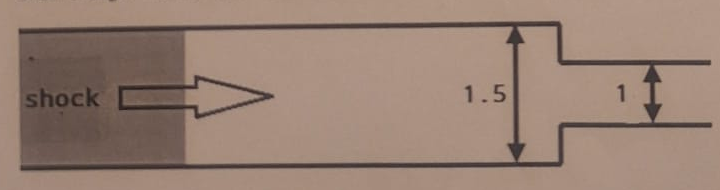
\includegraphics[width=0.75\textwidth]{schema.png}
  \caption{Schema della traccia: condotto largo di altezza \num{1.5} a sinistra, condotto stretto di altezza 1 a
  destra; l'urto viaggia verso destra.}
  \label{fig:schema}
\end{figure}

%==============================================================================
\section{Lettura del testo e dati}
Il gas è aria, gas perfetto con $\gamma=\num{1.4}$ ($\delta=(\gamma-1)/2=\num{0.2}$) in tutto il condotto. Le
grandezze sono adimensionali, riferite allo stato in quiete: $p_0=1$, $a_0=1$, quindi $\rho_0=\gamma p_0/a_0^2=\num{1.4}$.
Nessuna lunghezza è assegnata: il piano $x$--$t$ si può disegnare solo con le velocità delle onde, che è tutto
ciò che serve perché il problema è autosimile (\S\,\ref{sec:topologia}).

Il dato sull'urto non è il suo Mach ma il \emph{Mach assoluto del gas a valle}, $M_1=u_1/a_1=\num{1.87}$: il
gas messo in moto dall'urto è supersonico rispetto al condotto. Il Mach dell'urto $\Ms=w/a_0$ va ricavato.
Il rapporto d'area è $A_1/A_2=\num{1.5}$ (condotto largo $A_1$ a sinistra, stretto $A_2$ a destra; per un
condotto piano il rapporto delle altezze è il rapporto delle aree).

Si chiede di quanto cambia l'intensità dell'urto passando nel condotto stretto: la misuro con il Mach
dell'urto e con il rapporto di pressione attraverso di esso.

Stati: 0 quiete; 1 dietro l'urto incidente (condotto largo); 2 all'ingresso del condotto stretto; 3 e 4 ai due
lati del contatto nel condotto stretto (3 a sinistra, dietro l'onda $\uma$; 4 a destra, dietro l'urto trasmesso).

%==============================================================================
\section{Modello e ipotesi}
\begin{itemize}
  \item \textbf{Eulero quasi-1D instazionario, non viscoso, gas perfetto con $\gamma$ costante.} Lontano dal
    gradino il condotto ha sezione costante e l'urto è piano: le grandezze sono uniformi su ogni sezione e il
    moto è 1D. Il modello quasi-1D dà il comportamento medio sulla sezione, non i dettagli 2D allo spigolo.
  \item \textbf{Brusca variazione d'area attraversata in modo istantaneo, stazionario e isentropico.} Il salto
    d'area ha lunghezza nulla rispetto alle distanze percorse dalle onde; appena l'urto lo ha superato, il gas
    che lo attraversa vede una geometria fissa. Se il gas 1 è supersonico anche in assoluto (lo è:
    $M_1=\num{1.87}$), fra le sezioni $A_1$ e $A_2$ si conservano portata, entalpia totale ed entropia: vale
    la legge delle aree con $p^0$ e $a^0$ uguali.
  \item \textbf{Nuovo problema di Riemann nel condotto stretto.} Il gas che esce dal salto d'area (stato 2)
    incontra, nell'istante e nel punto d'arrivo dell'urto, il gas in quiete (stato 0) del condotto stretto: la
    discontinuità 2\,|\,0 è un problema di Riemann.
\end{itemize}

%==============================================================================
\section{Analisi qualitativa}
\textbf{Il condotto largo non riceve informazione.} Il gas 1 è supersonico ($u_1>a_1$): anche le
caratteristiche $\uma$, le sole che potrebbero portare a monte la notizia del gradino, sono trascinate verso
destra. Un'onda riflessa che risale il condotto largo può esistere solo se la contrazione non lascia passare
la portata (strozzamento): allora il gradino agirebbe in parte come una parete e rifletterebbe un urto $\uma$
capace di risalire la corrente. Lo escludo se la legge delle aree ammette una soluzione supersonica in $A_2$,
cioè se $A_1/A_2\le\Ar(M_1)$ (verificato al \S\,\ref{sec:calcolo}).

\textbf{Il salto d'area comprime.} Una corrente supersonica che entra in un convergente rallenta e si comprime:
lo stato 2 ha $p_2>p_1$, $u_2<u_1$, e resta supersonico (stesso ramo della legge delle aree, perché senza urti
non si cambia ramo).

\textbf{Il condotto stretto è un tubo d'urto.} Il gas 2, più compresso, fa da pistone sul gas in quiete
nel condotto stretto: nascono un \textbf{urto trasmesso} $\upa$ e un \textbf{contatto}. Per raccordare lo stato 2,
che ha velocità minore dello stato dietro l'urto e pressione molto maggiore, serve un'onda $\uma$ che acceleri
e decomprima il gas: mi aspetto un'\textbf{espansione} (da verificare dopo il calcolo). Con $u_2>a_2$ anche
questa espansione è trascinata verso destra, lontano dal gradino.

\textbf{Attesa sull'intensità.} In un convergente un'onda di compressione si intensifica: l'urto trasmesso deve
essere più forte dell'incidente.

%==============================================================================
\section{Topologia del campo}\label{sec:topologia}
Prima dell'arrivo c'è solo l'urto incidente $\upa$ fra 1 (sinistra) e 0 (destra). Dall'arrivo dell'urto sul
gradino ($x=0$, $t=0$) tutte le onde partono dallo stesso punto: il campo è \textbf{autosimile} e fatto solo di
stati uniformi, rette e un ventaglio centrato.
\begin{itemize}
  \item Condotto largo ($x<0$): stato 1 uniforme, invariato.
  \item Salto d'area ($x=0$): collegamento stazionario $1\to2$.
  \item Condotto stretto ($x>0$): stato 2 | \textbf{espansione centrata $\uma$} | stato 3 | \textbf{contatto}
    | stato 4 | \textbf{urto trasmesso $\upa$} | stato 0.
\end{itemize}
Non ci sono zone d'interazione a due famiglie: il ventaglio è un'onda semplice con caratteristiche $\uma$
semirette, e ogni altra regione è uniforme.

%==============================================================================
\section{Bilancio equazioni/incognite}
Noti 0 e 1, le incognite sono lo stato 2 (3 grandezze), l'intensità dell'onda $\uma$ e quella dell'urto
trasmesso, cioè $p^*$ e $u^*$ comuni ai due lati del contatto, più le due densità $\rho_3$, $\rho_4$. Le equazioni
sono: conservazione di portata, entalpia totale ed entropia nel salto d'area (3); invariante $a+\delta u$ e
isentropia attraverso l'espansione (2); Rankine--Hugoniot attraverso l'urto trasmesso (3, una delle quali
fissa la sua velocità $w_t$, incognita in più). Il conto torna: il condotto stretto è un problema di Riemann
standard con stato sinistro 2 noto, perché lo stato 2 non dipende da ciò che accade a valle (gas 2 supersonico).

%==============================================================================
\section{Scorciatoie fisiche}
\begin{itemize}
  \item \textbf{$\Ms$ esplicito dal Mach a valle.} Invece di iterare sulla velocità dell'urto, le relazioni di salto
    danno $M_1$ in funzione di $\Ms$ e si invertono con un'equazione di secondo grado in $\Ms^2$
    (\S\,\ref{sec:calcolo}).
  \item \textbf{Disaccoppiamento.} Il gas 1 e il gas 2 sono supersonici: il salto d'area si risolve con la sola
    legge delle aree, e il problema di Riemann nel condotto stretto non può modificarlo.
\end{itemize}

%==============================================================================
\section{Calcolo}\label{sec:calcolo}

\subsection{Urto incidente (stato 1)}
Nel riferimento dell'urto ($u_0=0$) la conservazione della massa e il rapporto delle temperature danno
\[
  \frac{u_1}{a_0}=\left(1-\frac{\rho_0}{\rho_1}\right)\Ms=\frac{2}{\gamma+1}\left(\Ms-\frac1{\Ms}\right),\qquad
  \frac{a_1^2}{a_0^2}=\frac{T_1}{T_0}=\frac{\left[2\gamma\Ms^2-(\gamma-1)\right]\left[(\gamma-1)\Ms^2+2\right]}{(\gamma+1)^2\Ms^2},
\]
quindi $M_1^2=u_1^2/a_1^2=4(\Ms^2-1)^2\big/\{[2\gamma\Ms^2-(\gamma-1)][(\gamma-1)\Ms^2+2]\}$, cioè, con $X=\Ms^2$,
\[
  \left[4-2\gamma(\gamma-1)M_1^2\right]X^2-\left[8+\left(4\gamma-(\gamma-1)^2\right)M_1^2\right]X+4+2(\gamma-1)M_1^2=0 .
\]
Delle due radici solo una ha $\Ms>1$ (l'altra dà $\Ms\approx\num{0.50}$, non è un urto):
\[
  \Ms=\num{17.99},\qquad w_i=\Ms a_0=\num{17.99}.
\]
Il coefficiente di $X^2$ si annulla per $M_1=\sqrt{2/[\gamma(\gamma-1)]}=\num{1.89}$, il Mach assoluto massimo
dietro un urto mobile in gas fermo (urto infinitamente forte): $M_1=\num{1.87}$ è vicino a questo limite, quindi
l'urto è fortissimo. Per lo stesso motivo $\Ms$ è molto sensibile alla seconda cifra decimale di $M_1$.

Stato 1 da Rankine--Hugoniot:
\[
  \frac{p_1}{p_0}=\frac{2\gamma\Ms^2-(\gamma-1)}{\gamma+1}=\num{377},\qquad
  \frac{\rho_1}{\rho_0}=\frac{(\gamma+1)\Ms^2}{(\gamma-1)\Ms^2+2}=\num{5.91},\qquad
  \frac{a_1}{a_0}=\sqrt{\frac{p_1/p_0}{\rho_1/\rho_0}}=\num{7.99},
\]
\[
  u_1=w_i\left(1-\frac{\rho_0}{\rho_1}\right)=\num{14.94},\qquad M_1=\frac{u_1}{a_1}=\num{1.87}\ \text{(come da dato)},
\]
con $\rho_1=\num{8.27}$.

\subsection{Salto d'area (stato 2)}
Per la legge delle aree
\[
  \Ar(M)=\frac{A}{A^*}=\frac1M\left[\frac{2}{\gamma+1}\left(1+\delta M^2\right)\right]^{\frac{\gamma+1}{2(\gamma-1)}},
  \qquad \frac{A_1}{A^*}=\Ar(M_1)=\num{1.519}>\frac{A_1}{A_2}=\num{1.5}:
\]
la sezione critica della corrente 1 è più piccola del condotto stretto, quindi tutta la portata passa senza
strozzamento e non nasce un urto riflesso. Nel condotto stretto
\[
  \frac{A_2}{A^*}=\frac{\Ar(M_1)}{A_1/A_2}=\num{1.013}\quad\Rightarrow\quad M_2=\num{1.126}\ \text{(ramo supersonico)}.
\]
Con $p^0$ e $a^0$ conservati, da $p^0/p=(1+\delta M^2)^{\gamma/(\gamma-1)}$ e $(a^0/a)^2=1+\delta M^2$:
\[
  p_2=p_1\left(\frac{1+\delta M_1^2}{1+\delta M_2^2}\right)^{\frac{\gamma}{\gamma-1}}=\num{1094},\qquad
  a_2=a_1\sqrt{\frac{1+\delta M_1^2}{1+\delta M_2^2}}=\num{9.30},\qquad u_2=M_2a_2=\num{10.48},
\]
con $\rho_2=\num{17.7}$. La pressione quasi triplica ($p_2/p_1=\num{2.90}$) e la velocità cala.

\subsection{Condotto stretto: problema di Riemann fra 2 (sinistra) e 0 (destra)}
\textbf{Curve delle due onde.} L'onda destra, in gas fermo, è un urto se $u>0$. Le relazioni di salto danno
$u-u_0=\frac{2a_0}{\gamma+1}\left(\Mr-\frac1{\Mr}\right)$, equazione di secondo grado in $\Mr$:
\[
  \Mr=Y+\sqrt{1+Y^2},\quad Y=\frac{\gamma+1}{4}\,\frac{u-u_0}{a_0},\qquad
  p_{\rm dx}(u)=p_0\left[1+\frac{2\gamma}{\gamma+1}\left(\Mr^2-1\right)\right].
\]
L'onda sinistra è un'espansione se $u>u_2$ ($a+\delta u$ uniforme e isentropia), un urto se $u<u_2$ (stessa
relazione con $(u_2-u)/a_2$ e $p_2$):
\[
  p_{\rm sx}(u)=p_2\left[1-\delta\,\frac{u-u_2}{a_2}\right]^{\frac{2\gamma}{\gamma-1}}\quad(u>u_2).
\]
\textbf{Primo tentativo} isentropico sulla velocità del contatto:
\[
  z=\frac{a_0}{a_2}\left(\frac{p_2}{p_0}\right)^{\frac{\gamma-1}{2\gamma}}=\num{0.292},\qquad
  u^{(0)}=\frac{z\,(a_2+\delta u_2)-(a_0-\delta u_0)}{\delta(1+z)}=\num{9.01}.
\]
Il primo tentativo è lontano dalla soluzione (e dà $u^{(0)}<u_2$, cioè un urto a sinistra): l'urto destro ha
$\Mr\approx19$ e l'ipotesi isentropica su di esso non regge. Aggiorno $u$ intersecando le tangenti alle due
curve $p_{\rm sx}(u)$ e $p_{\rm dx}(u)$:
\begin{table}[H]
  \centering
  \begin{tabular}{ccccc}
    \toprule
    passo & $u$ & onda sinistra & $p_{\rm sx}$ & $p_{\rm dx}$ \\
    \midrule
    0 & \num{9.01}  & urto        & \num{1359} & \num{139} \\
    1 & \num{14.36} & espansione  & \num{594}  & \num{349} \\
    2 & \num{16.04} & espansione  & \num{448}  & \num{435} \\
    3 & \num{16.148} & espansione & \num{440.27} & \num{440.23} \\
    \bottomrule
  \end{tabular}
\end{table}
Al passo 3 $|p_{\rm sx}-p_{\rm dx}|/p\approx10^{-4}$: fisicamente zero. Configurazione \textbf{RCS}:
\[
  u^*=\num{16.15},\qquad p^*=\num{440}.
\]

\textbf{Stato 3} (coda dell'espansione, $a+\delta u$ uniforme nell'onda $\uma$):
\[
  a_3=a_2-\delta\left(u^*-u_2\right)=\num{8.17},\qquad
  p_3=p_2\left(\frac{a_3}{a_2}\right)^{\frac{2\gamma}{\gamma-1}}=\num{440},\qquad
  \rho_3=\frac{\gamma p_3}{a_3^2}=\num{9.24},\qquad M_3=\num{1.98}.
\]
Il ventaglio ha testa $u_2-a_2=\num{1.18}$ e coda $u_3-a_3=\num{7.98}$.

\textbf{Stato 4} (dietro l'urto trasmesso):
\[
  \Mr=\num{19.43},\qquad \frac{p_4}{p_0}=\frac{2\gamma\Mr^2-(\gamma-1)}{\gamma+1}=\num{440},\qquad
  \frac{\rho_4}{\rho_0}=\frac{(\gamma+1)\Mr^2}{(\gamma-1)\Mr^2+2}=\num{5.92},
\]
\[
  w_t=u_0+\Mr a_0=\num{19.43},\qquad a_4=\num{8.62},\qquad M_4=\frac{u^*}{a_4}=\num{1.87},
\]
con $\rho_4=\num{8.29}$.

\subsection{Variazione d'intensità}
\[
  \frac{\Ms^{\rm trasm}}{\Ms^{\rm inc}}=\frac{w_t}{w_i}=\num{1.080},\qquad
  \frac{p_4/p_0}{p_1/p_0}=\num{1.167},\qquad
  \frac{p_4-p_0}{p_1-p_0}=\num{1.167}.
\]
L'urto si \textbf{rinforza}: il suo Mach passa da \num{17.99} a \num{19.43} (+8\,\%) e il salto di pressione da
\num{377} a \num{440} (+17\,\%); la velocità del gas dietro l'urto passa da \num{14.94} a \num{16.15}.

%==============================================================================
\section{Verifiche a posteriori}
\begin{itemize}
  \item Urto incidente: $\Ms=\num{17.99}>1$, $s_1/s_0=\num{31.4}>1$, e $u_1/a_1=\num{1.87}$ restituisce il dato. Verificata.
  \item Gas 1 supersonico: $u_1-a_1=\num{6.95}>0$, nessuna onda risale il condotto largo. Verificata.
  \item Salto d'area senza strozzamento: $\Ar(M_1)=\num{1.519}>A_1/A_2$; portata $\rho_1u_1A_1=\rho_2u_2A_2$,
    $h^0_1=h^0_2$, $s_1=s_2$. Verificata.
  \item Gas 2 supersonico: $u_2-a_2=\num{1.18}>0$, il ventaglio si stacca dal gradino e non perturba il collegamento
    stazionario. Verificata.
  \item Natura dell'onda sinistra: $u^*>u_2$ e $p^*<p_2$, espansione come atteso. Verificata.
  \item Ordine delle onde: testa \num{1.18} $<$ coda \num{7.98} $<$ contatto \num{16.15} $<$ urto \num{19.43}. Verificata.
  \item Urto trasmesso: $\Mr=\num{19.43}>1$, $s_4/s_0=\num{36.5}>1$. Verificata.
  \item Contatto: $p_3=p_4$, $u_3=u_4$, $\rho_3\neq\rho_4$; $a>0$, $p>0$ ovunque. Verificata.
\end{itemize}

%==============================================================================
\section{Risultati}
\begin{table}[H]
  \centering
  \begin{tabular}{clrrrrr}
    \toprule
    Stato & Posizione & $p$ & $\rho$ & $u$ & $a$ & $M$ \\
    \midrule
    0 & quiete & 1 & \num{1.40} & 0 & 1 & 0 \\
    1 & dietro l'urto incidente ($A_1$) & \num{377} & \num{8.27} & \num{14.94} & \num{7.99} & \num{1.87} \\
    2 & ingresso del condotto stretto & \num{1094} & \num{17.7} & \num{10.48} & \num{9.30} & \num{1.13} \\
    3 & coda dell'espansione & \num{440} & \num{9.24} & \num{16.15} & \num{8.17} & \num{1.98} \\
    4 & dietro l'urto trasmesso & \num{440} & \num{8.29} & \num{16.15} & \num{8.62} & \num{1.87} \\
    \bottomrule
  \end{tabular}
\end{table}
\begin{table}[H]
  \centering
  \begin{tabular}{lll}
    \toprule
    Onda & Velocità nel piano $x$--$t$ & Intensità \\
    \midrule
    urto incidente $\upa$ & $w_i=\num{17.99}$ & $\Ms=\num{17.99}$, $p_1/p_0=\num{377}$ \\
    salto d'area (stazionario) & $x=0$ & $p_2/p_1=\num{2.90}$ \\
    espansione $\uma$ & testa \num{1.18}, coda \num{7.98} & $p_3/p_2=\num{0.40}$ \\
    contatto & $u^*=\num{16.15}$ & $\rho_3/\rho_4=\num{1.11}$ \\
    urto trasmesso $\upa$ & $w_t=\num{19.43}$ & $\Ms=\num{19.43}$, $p_4/p_0=\num{440}$ \\
    \midrule
    \multicolumn{3}{l}{Variazione d'intensità: $\Ms$ $\times\num{1.080}$ (+8\,\%), salto di pressione $\times\num{1.167}$ (+17\,\%)} \\
    \bottomrule
  \end{tabular}
\end{table}

%==============================================================================
\section{Rappresentazioni}

\begin{figure}[H]
  \centering
  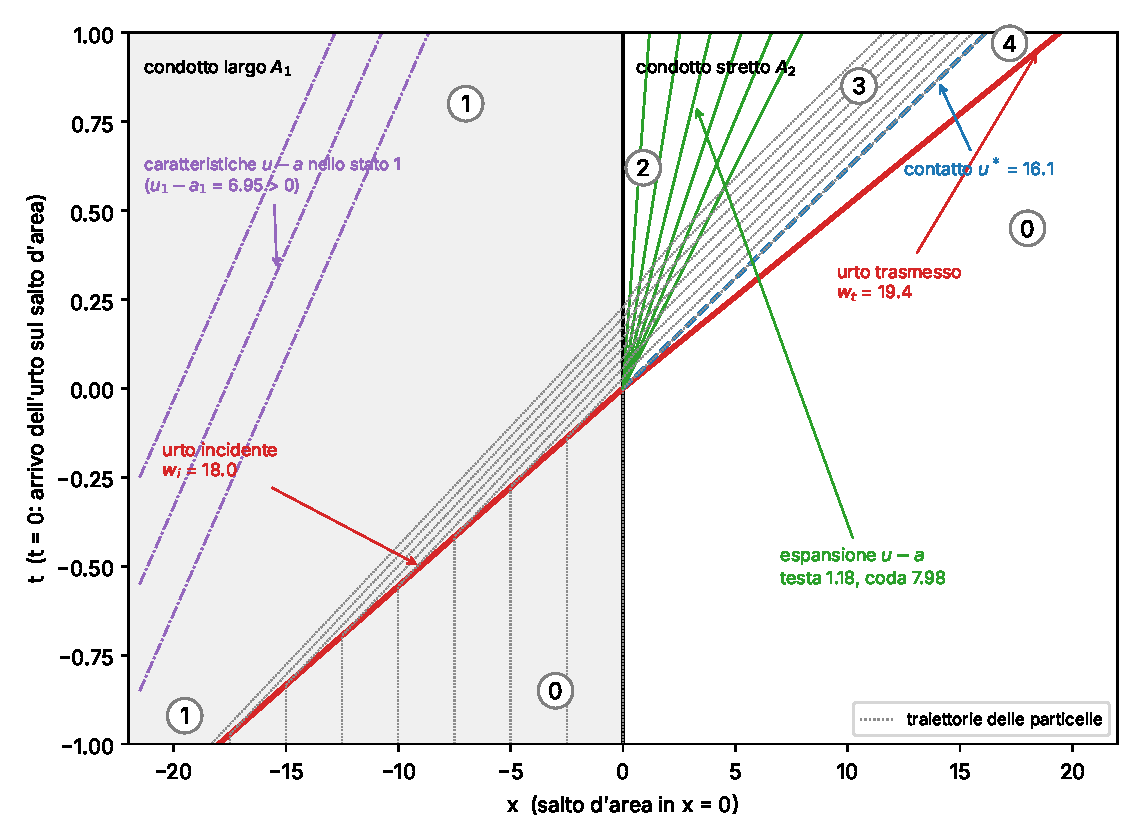
\includegraphics[width=0.88\textwidth]{xt.pdf}
  \caption{Piano $x$--$t$ con le velocità calcolate (scala dei tempi arbitraria: nessuna lunghezza è assegnata).
  Origine nell'arrivo dell'urto sul salto d'area.}
  \label{fig:xt}
\end{figure}
\textbf{Piano $x$--$t$.} Per $t<0$ c'è solo l'urto incidente: le particelle, ferme nello stato 0, partono
quando l'urto le raggiunge. Le caratteristiche $\uma$ nello stato 1 (tratto-punto) hanno pendenza
positiva: il condotto largo non sa nulla del gradino, e per $x<0$ lo stato 1 resta invariato anche dopo
$t=0$. Dal punto d'arrivo partono, nel condotto stretto, il ventaglio d'espansione $\uma$ (tutto con pendenza
positiva, la testa appena inclinata rispetto alla verticale), il contatto e l'urto trasmesso, più veloce
dell'incidente (retta più inclinata verso l'asse $x$). Fra il gradino e la testa del ventaglio c'è lo stato 2,
che si allarga nel tempo. Le traiettorie delle particelle rallentano attraversando il gradino ($u_1\to u_2$),
accelerano nel ventaglio e procedono con $u^*$ nello stato 3; quelle dello stato 4 sono gas del condotto stretto
messo in moto dall'urto trasmesso.

\begin{figure}[H]
  \centering
  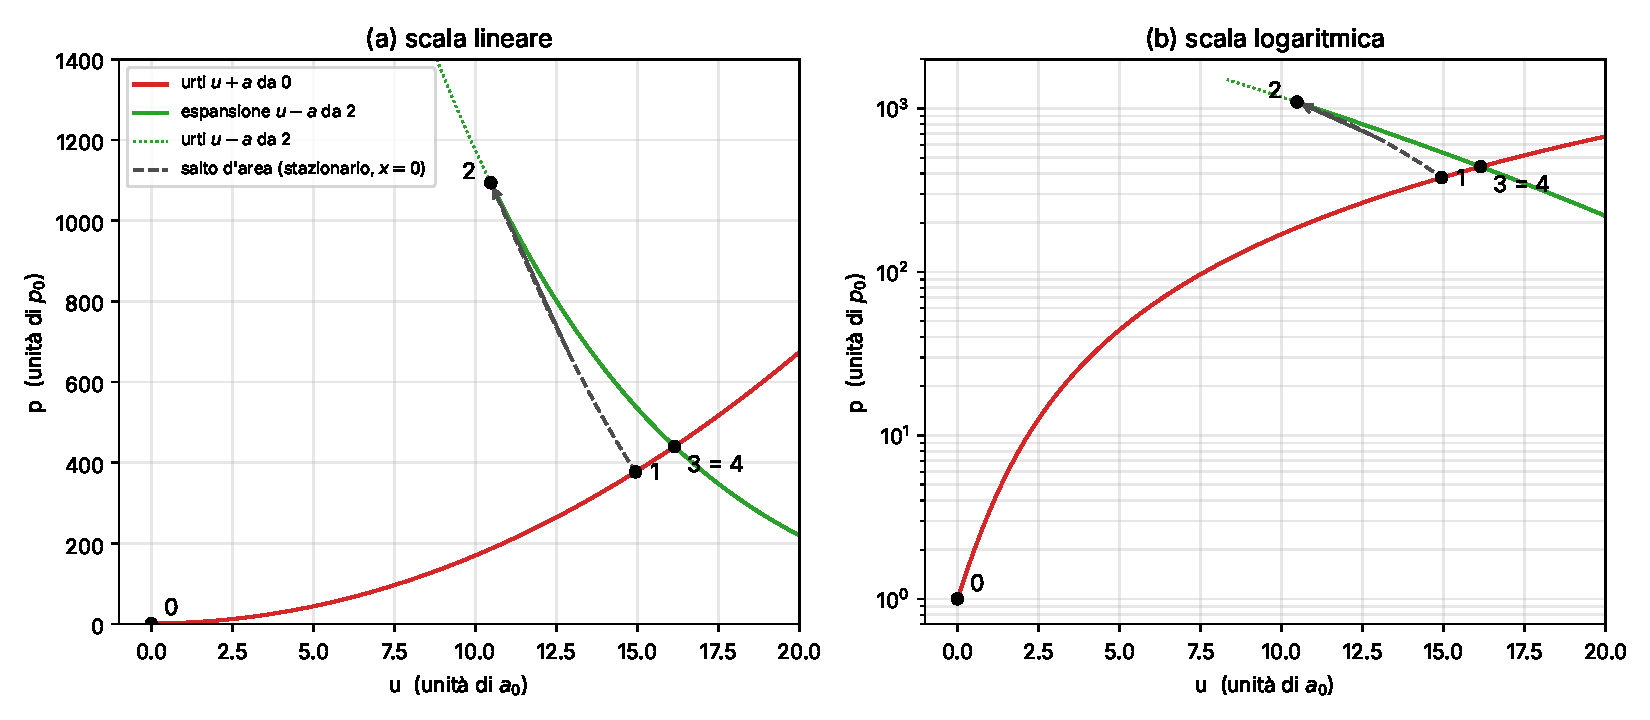
\includegraphics[width=\textwidth]{pu.pdf}
  \caption{Piano $p$--$u$ in scala lineare (a) e logaritmica (b). Il tratteggio $1\to2$ è il collegamento
  stazionario nel salto d'area (al variare di $A$ da $A_1$ ad $A_2$), non un'onda.}
  \label{fig:pu}
\end{figure}
\textbf{Piano $p$--$u$.} Le pressioni vanno da 1 a circa \num{1100}, quindi riporto entrambe le scale. Lo stato 1
sta sulla curva degli urti $\upa$ uscente da 0. Il salto d'area porta 1 in 2, più in alto e a sinistra
(compressione con rallentamento). Da 2 la curva d'espansione $\uma$ scende verso destra e incontra di nuovo la
curva degli urti uscente da 0 nel punto $3=4$, \emph{sopra} il punto 1: è il rinforzo dell'urto trasmesso
rispetto all'incidente. Il contatto non si vede ($\rho_3\neq\rho_4$). La scala lineare mostra quanto lo stato 2
sta sopra gli altri e quanto i punti 1 e $3=4$ sono vicini sulla stessa curva; la scala logaritmica rende
leggibili insieme lo stato in quiete e gli stati dietro gli urti, e i rapporti di pressione delle singole onde.

%==============================================================================
\section{Discussione fisica}
\textbf{Perché l'urto si rinforza.} Il gas 1 entra nel condotto stretto rallentando e comprimendosi: lo stato 2
è un ``driver'' a pressione quasi tripla rispetto al gas 1. Nel condotto stretto questo driver si espande verso
il gas in quiete come in un tubo d'urto, e la pressione che riesce a mantenere dietro l'urto ($p^*=\num{440}$) è
maggiore di $p_1$. È l'intensificazione di un'onda di compressione in un convergente.

\textbf{Il risultato relativo non dipende dalla forza dell'urto.} $M_1=\num{1.87}$ è vicino al limite
\num{1.89} degli urti fortissimi: $\Ms$ dipende molto dalla seconda cifra decimale di $M_1$, ma i rapporti
$w_t/w_i\approx\num{1.08}$ e $(p_4-p_0)/(p_1-p_0)\approx\num{1.17}$ quasi no. Per urti fortissimi la
pressione a monte è trascurabile e il campo dietro l'urto dipende solo da $\gamma$ (e $M_1\to\num{1.89}$): il
rinforzo dipende solo da $\gamma$ e da $A_1/A_2$.

\textbf{Margine sullo strozzamento.} $\Ar(M_1)=\num{1.519}$ supera $A_1/A_2=\num{1.5}$ di poco più dell'1\,\%. Basta
una perdita di pressione totale di circa l'1\,\% nel salto d'area per far salire $A^*$ oltre $A_2$: la
contrazione strozzerebbe e dal gradino partirebbe un urto $\uma$ che risale il condotto largo, con un campo
diverso (sezione sonica in $A_2$). Nella realtà allo spigolo vivo la corrente supersonica forma urti obliqui
e perde pressione totale, quindi questa situazione è plausibile: il risultato isentropico quasi-1D va letto
come il caso ideale.

\textbf{Contatto e strato entropico.} Il gas 3 ha attraversato l'urto incidente e poi solo trasformazioni
isentropiche; il gas 4 ha attraversato un urto più forte: $s_4>s_3$, $a_4>a_3$ e $\rho_4<\rho_3$ a pari $p$. Il
contatto separa gas con entropia diversa, come avviene ogni volta che un urto cambia intensità.

\textbf{Limiti del modello.} Il modello trascura la fase 2D dell'interazione (riflessione dell'urto sulla corona
del gradino, diffrazione allo spigolo, urto trasmesso inizialmente curvo), che conta solo nei primi istanti. Con
$\Ms\approx18$ il rapporto delle temperature $T_1/T_0\approx64$ è fuori dal campo del gas perfetto con $\gamma=\num{1.4}$
(dissociazione e ionizzazione dell'aria): il calcolo vale come esercizio a $\gamma$ costante.

\end{document}
